\documentclass{article}
\usepackage{tikz}

\begin{document}

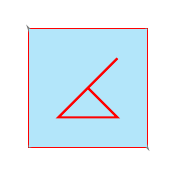
\begin{tikzpicture}[scale=1.5]
    % Define coordinates for the main points of the diamond
    \coordinate (A) at (0,0);
    \coordinate (B) at (1,0);
    \coordinate (C) at (1,1);
    \coordinate (D) at (0,1);

    % Draw the main diamond shape
    \draw[red, thick] (A) -- (B) -- (C) -- (D) -- cycle;

    % Define coordinates for the additional points
    \coordinate (E) at (0.5, 0.5);
    \coordinate (F) at (0.75, 0.75);
    \coordinate (G) at (0.25, 0.25);
    \coordinate (H) at (0.75, 0.25);
    \coordinate (I) at (0.25, 0.75);

    % Draw the additional lines
    \draw[gray, thick] (A) -- (E) -- (B) -- (F) -- (C) -- (G) -- (D) -- (H) -- (A);
    \draw[gray, thick] (E) -- (F) -- (G) -- (H) -- (E);

    % Fill the shape with a light blue color
    \fill[cyan!30] (A) -- (B) -- (C) -- (D) -- cycle;
    \fill[cyan!30] (E) -- (F) -- (G) -- (H) -- cycle;

    % Draw the outline of the additional shape in red
    \draw[red, thick] (E) -- (F) -- (G) -- (H) -- cycle;
\end{tikzpicture}

\end{document}